\begin{center}
\fbox{\fbox{\parbox{6.5in}{\centering
\begin{flushleft}


\vspace{2mm}
\hspace{5mm}
\textbf{\underline{Tähistuste tähendused}}

\vspace{2mm}
\hspace{5mm}
Sirgete \textbf{paralleelsust} tähistatakse sümboliga: $\parallel$

\vspace{2mm}
\hspace{5mm}
Näiteks: Sirge $a$ on paralleelne sirgega $b$. Tähistus: $a \parallel b$

\vspace{5mm}
\hspace{5mm}
Sirgete \textbf{lõikumist} tähistatakse sümboliga: $\cancel{\parallel}$ (kuna mitte paralleelsed sirged lõikuvad).

\vspace{2mm}
\hspace{5mm}
Näiteks: Sirge $a$ lõikub sirgega $b$. Tähistus: $a \cancel{\parallel} b$


\vspace{5mm}
\hspace{5mm}
Sirgete \textbf{ristumist} tähistatakse sümboliga: $\perp$

\vspace{2mm}
\hspace{5mm}
Näiteks: Sirge $a$ on risti sirgega $b$. Tähistus: $a \perp b$



\vspace{2mm}
\hspace{5mm}
\textbf{\underline{Paralleelide aksioom}}

\vspace{2mm}
\hspace{5mm}
Väljaspool sirget asetsevat punkti läbib ainult üks sirge, mis on paralleelne antud sirgega.

\begin{center}
\vspace{2mm}
\hspace{5mm}
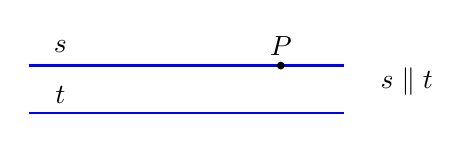
\begin{tikzpicture}[scale=0.4]
\draw[line width=0.3mm, blue] (0,0) to (10,0);
\draw[line width=0.3mm, blue] (0,-1.5) to (10,-1.5);
\node at(8,0)[circle,fill, black, inner sep=1pt]{};
\node[above] at(8,0) {$P$};
\node[above] at (1, 0.1) {$s$};
\node[above] at (1, -1.5) {$t$};
\node at (12,-0.5) {$s \parallel t$};
\end{tikzpicture}
\end{center}


\vspace{2mm}
\hspace{5mm}
\textbf{Teoreemid}

\vspace{2mm}
\hspace{5mm}
1) Kui kaks sirget on paralleelsed kolmandaga, siis on nad paralleelsed teineteisega. 

\begin{center}
\vspace{2mm}
\hspace{5mm}
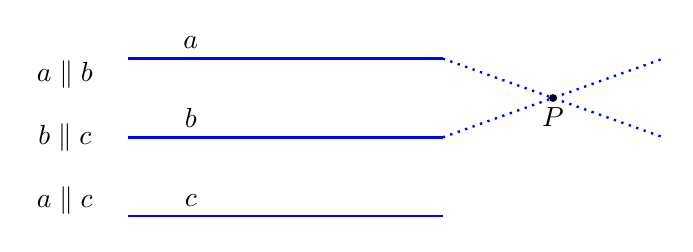
\begin{tikzpicture}[scale=0.4]
\node[above] at (2,0) {$a$};
\draw[line width=0.3mm, blue] (0,0) to (10,0);
\node[above] at (2,-2.5){$b$};
\draw[line width=0.3mm, blue] (0,-2.5) to (10,-2.5);
\draw[dotted, line width=0.3mm, blue] (10,0) to (17,-2.5);
\draw[dotted, line width=0.3mm, blue] (10,-2.5) to (17, 0);
\node at (13.5, -1.25)[circle,fill, black, inner sep=1pt]{};
\node[below] at (13.5, -1.25){$P$};
\node[above] at (2,-5){$c$};
\draw[line width=0.3mm, blue] (0,-5) to (10,-5);
\node at (-2,-0.5){$a \parallel b$};
\node at (-2, -2.5){$b \parallel c$};
\node at(-2,-4.5){$a \parallel c$};


\end{tikzpicture}
\end{center}

\vspace{2mm}
\hspace{5mm}
2) Kui sirge lõikab ühte kahest paralleelsest sirgest, siis lõikab ta ka teist.

\begin{center}
\vspace{2mm}
\hspace{5mm}
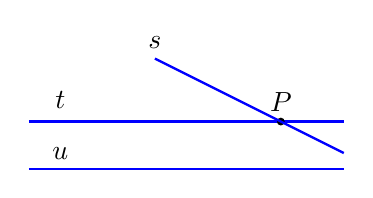
\begin{tikzpicture}[scale=0.4]
\draw[line width=0.3mm, blue] (0,0) to (10,0);
\draw[line width=0.3mm, blue] (0,-1.5) to (10,-1.5);
\node at(8,0)[circle,fill, black, inner sep=1pt]{};
\node[above] at(8,0) {$P$};
\node[above] at (1, 0.1) {$t$};
\node[above] at (1, -1.5) {$u$};

\draw[line width=0.3mm, blue] (4,2) to (10,-1);
\node[above] at (4,2){$s$};
\end{tikzpicture}
\end{center}

\vspace{2mm}
\hspace{5mm}
3) Kui kaks sirget on risti ühe ja sama sirgega, siis on need sirged paralleelsed.

\begin{center}
\vspace{2mm}
\hspace{5mm}
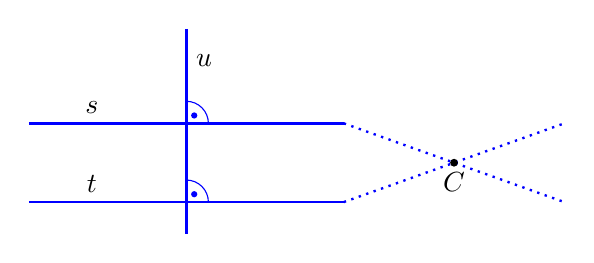
\begin{tikzpicture}[scale=0.4]
\node[above] at (2,0) {$s$};
\draw[line width=0.3mm, blue] (0,0) to (10,0);
\node[above] at (2,-2.5){$t$};
\draw[line width=0.3mm, blue] (0,-2.5) to (10,-2.5);
\draw[dotted, line width=0.3mm, blue] (10,0) to (17,-2.5);
\draw[dotted, line width=0.3mm, blue] (10,-2.5) to (17, 0);
\node at (13.5, -1.25)[circle,fill, black, inner sep=1pt]{};
\node[below] at (13.5, -1.25){$C$};

\draw[line width=0.3mm, blue] (5,3) to (5, -3.5);
\node[right] at (5,2){$u$};
\draw[blue](5.7,0) arc(0:90:0.7cm);
\node at (5.25,0.25) [circle, fill,blue, inner sep=0.8pt]{};

\draw[blue](5.7,-2.5) arc(0:90:0.7cm);
\node at (5.25,-2.25) [circle, fill,blue, inner sep=0.8pt]{};

\end{tikzpicture}
\end{center}

\end{flushleft}
}}}
\end{center}

\pagebreak

\vspace{0.5cm}

\textbf{Märkmed}\\
\vspace{2mm}
\begin{mdframed}[style=graphpaper]
\vspace{21cm}
\end{mdframed}